%
% Kapitel2.tex
%
%
\chapter{Background}
This chapter details the principles of Distributed Acoustic Sensing (DAS), including the C-OTDR measurement principle, the components of the AP Sensing DAS hardware, and the functionality of the DAS Configurator application used for data acquisition and visualization. Then, it introduces the fundamentals of Machine Learning for image recognition, explaining key evaluation metrics derived from the confusion matrix, data augmentation techniques, and the basics of the PyTorch and Kornia libraries. The chapter concludes with a literature review that situates this work within the context of previous research on DAS-based activity detection.

\section{Distributed Acoustic Sensing}

Distributed Acoustic Sensing (DAS) transforms a standard fiber-optic cable into a dense array of thousands of virtual microphones. By sending pulses of laser light down the fiber and analyzing the coherent Rayleigh backscatter, a DAS system can detect minute physical disturbances acoustic vibrations or strain at any point along the cable's length. This enables precise localization and real-time monitoring of events over distances of several kilometers. Common applications include power-cable integrity checks, pipeline leak detection, train tracking, and perimeter security, where the system can continuously surveil and trigger alarms for anomalous activity. 

\subsection{Measurement Principle}

The current measuring principle behind the DAS is measurement of acoustic vibrations based on the Coherent Optical Time Domain Refractometry (C-OTDR). It measures the change in length and index of refraction of the fiber induced by the temperature changes and acoustic or seismic waves interacting with the cable~\cite{duckworth}. Laser is sent into the fiber and the backscattered light is detected and analyzed. 

\begin{figure}[h]
    \centering
    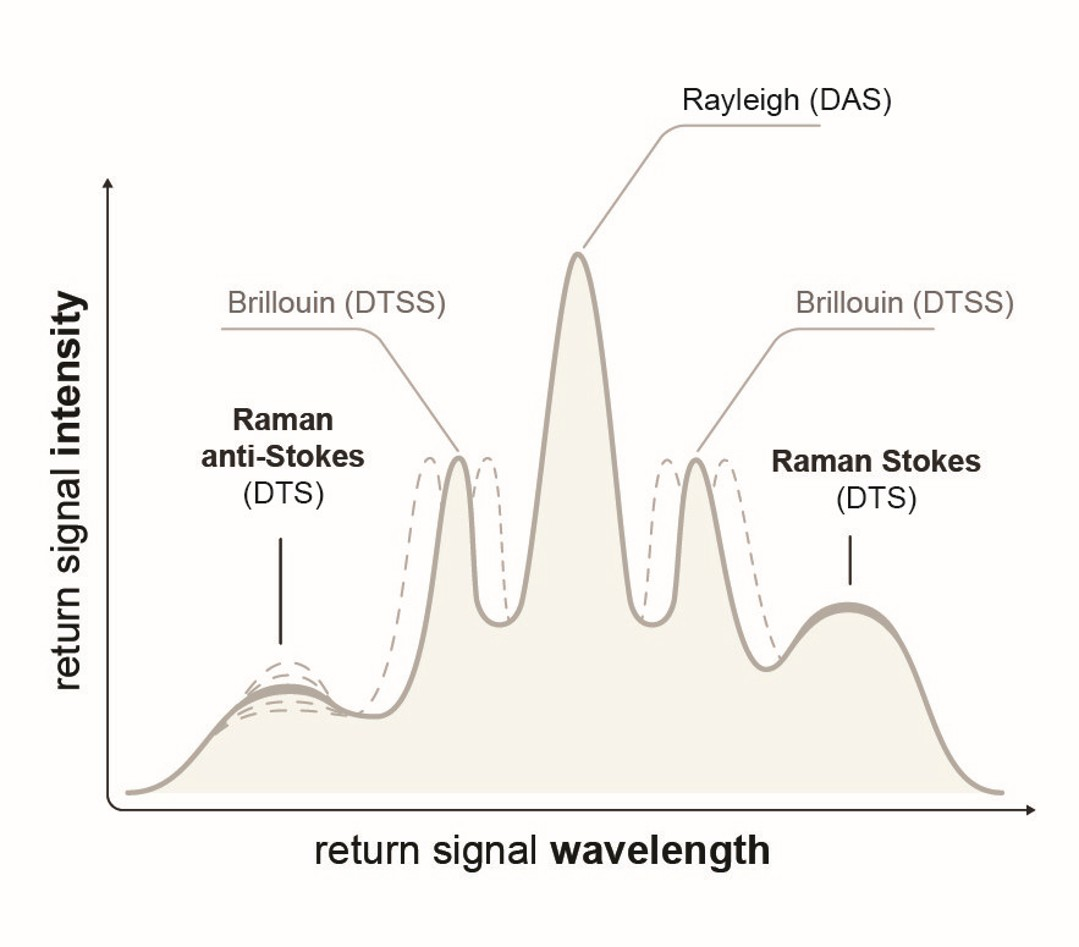
\includegraphics[width=0.7\linewidth]{Bilder/jpg/COTDR.jpg}
    \caption{Spectral signal intensity distribution of the backscattered light~\cite{DAS_Manual}}
    \label{COTDR}
\end{figure}
 
Spectral signal intensity distribution of the backscattered light from the fiber is shown in Figure~\ref{COTDR}. DAS systems work on the Rayleigh Backscattering which is the highest peak in the Figure. It is a small fraction of light scattered by microscopic variations in fibre's refractive index. By sending the short pulses of laser and measuring the backscattering Rayleigh signal as a function of time, signals are localized along the fiber~\cite{masoudi}.  

\begin{figure}[h]
    \centering
    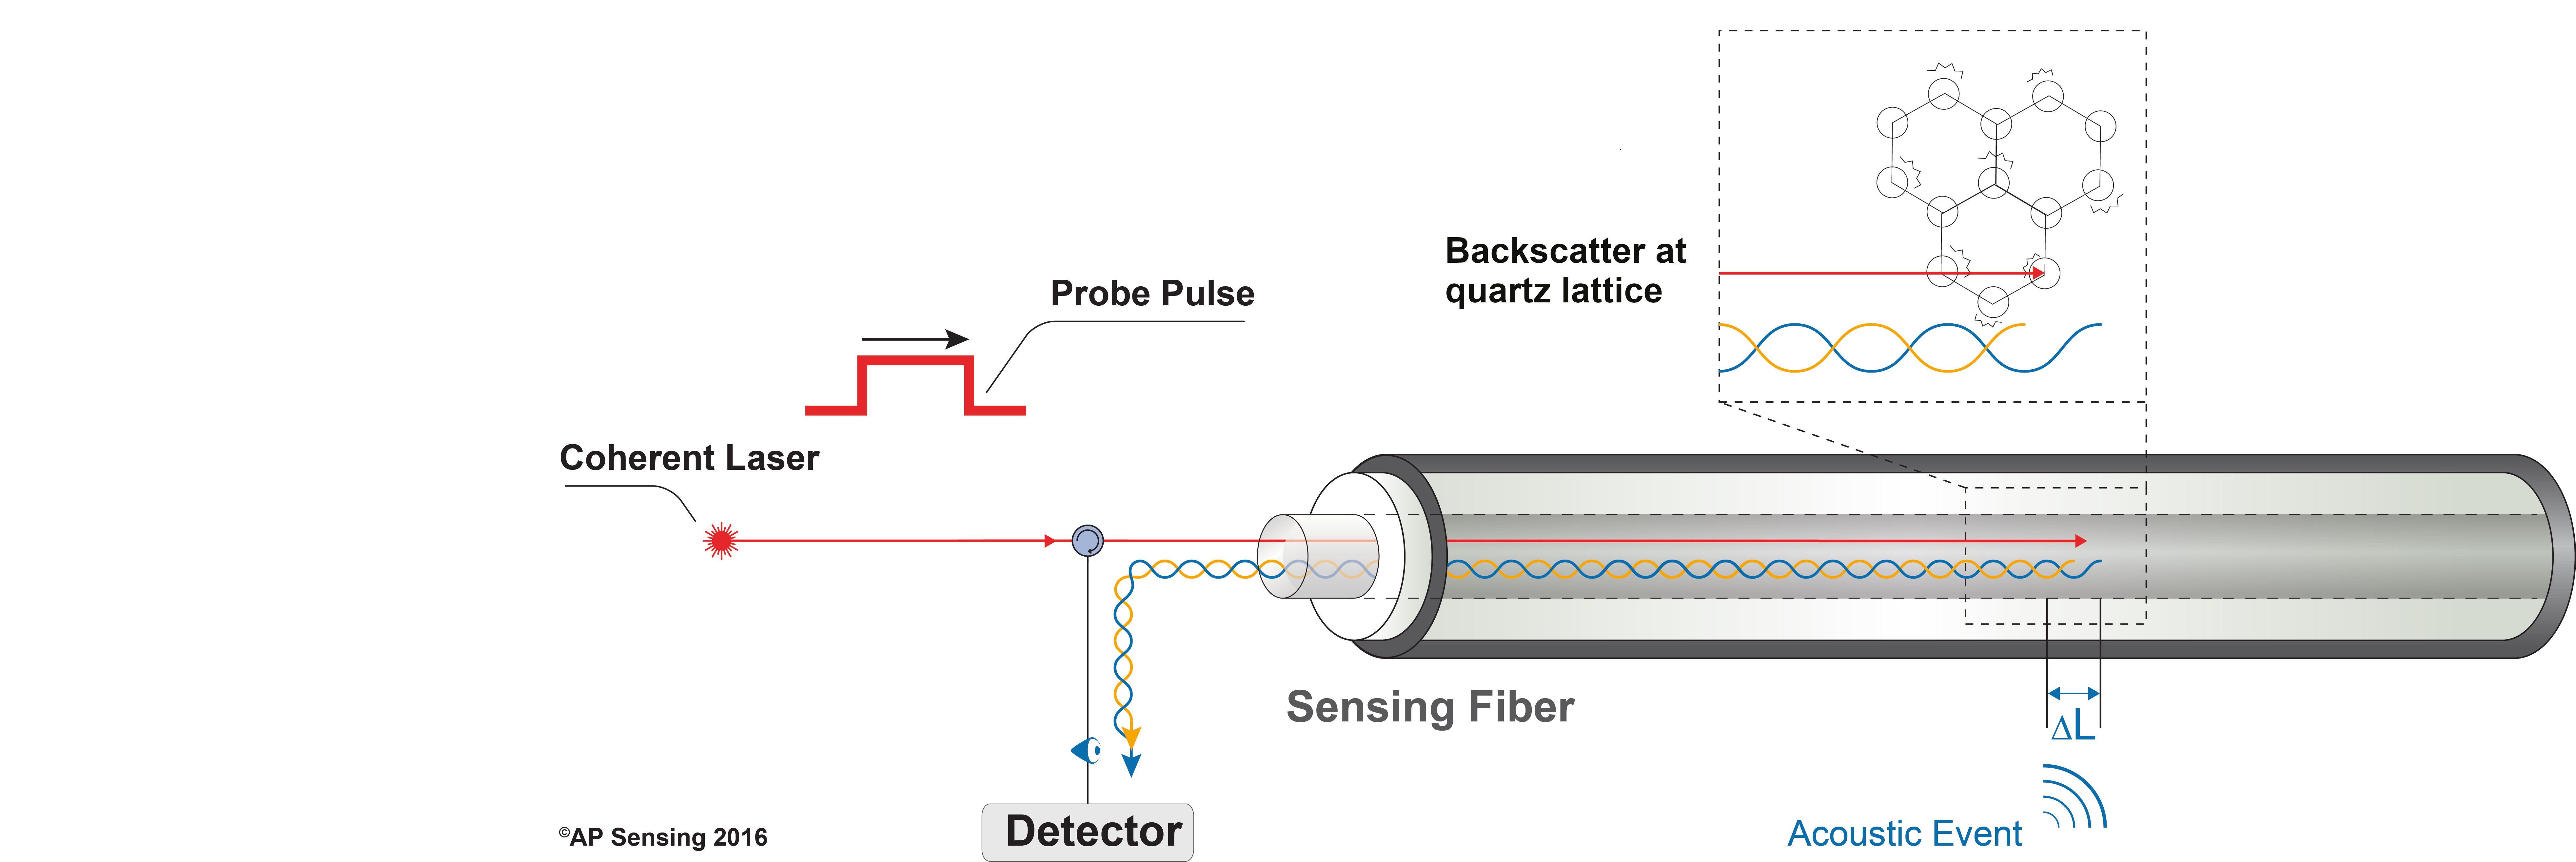
\includegraphics[width=0.7\linewidth]{Bilder/jpg/DAS_Acoustic_Event.jpg}
    \caption{Working principle of DAS system~\cite{DAS_Manual}}
    \label{DAS_working}
\end{figure}

Figure~\ref{DAS_working} shows how the laser is sent through the fiber optic cable and detected back after back scattering. When the acoustic event takes place, a tiny elongation or compression($\Delta L$) alters the phase relationship of the backscattered light signals. These signals are analyzed to show the frequency and amplitude disturbances. An Exact location of the acoustic event can be identified by measuring the time-dependent return of the light,  the same principle used in radar echos. 

\begin{figure}[h]
  \centering
  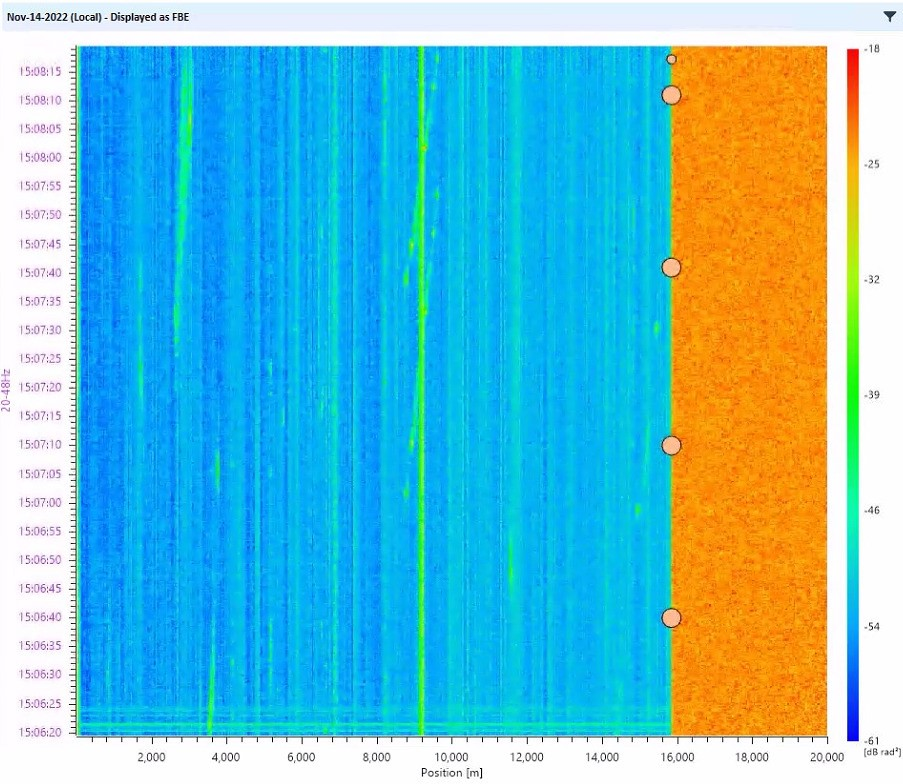
\includegraphics[width=0.7\linewidth]{Bilder/jpg/DAS Waterfall.jpg}
  \caption{Waterfall Diagram~\cite{Waterfall}}
  \label{DAS_waterfall}
\end{figure}

After digitizing and filtering the analog signals, the data can be processed and analyzed over distance and time and displayed in the form of a waterfall diagram as shown in the Figure~\ref{DAS_waterfall} where X-axis is the position on fiber and Y-axis is timestamp of recording. The data is recorded in the files in the HDF5 file format. The data from the HDF5 file is used to develop an algorithm which is used for the footsteps detection. Transforming the signal amplitude over time and in the frequency domain retrieves the acoustic event's frequency content. Using the acoustic event's location, amplitude, and frequency response, the system sets up an alarm for a potential threat-related activity. 

\subsection{AP Sensing DAS System}
There are two main components of the AP Sensing DAS system - the Interrogator Unit(IU) and the Digital Processing Unit(DPU). Figure~\ref{DAS} shows the IU(top) and DPU(bottom) which are the part of the DAS system.

\begin{figure}[h]
    \centering
    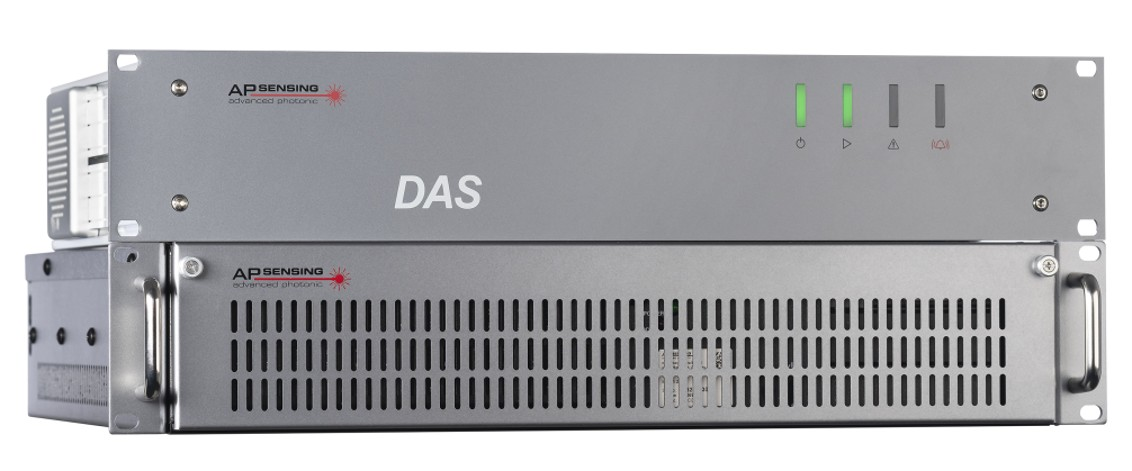
\includegraphics[width=\linewidth]{Bilder/jpg/DAS.jpg}
    \caption{AP Sensing DAS device~\cite{DAS_Manual}}
    \label{DAS}
\end{figure}

The IU(top) has the task of sending out highly coherent laser pulses into the fiber and thereby detecting the change in phase which is caused by Rayleigh backscattering. Analog signals containing the information in the form of frequency and amplitude are then sent to the DPU(bottom) for further processing. Figure~\ref{IU} shows the rear panel of the IU and all the ports present.

\begin{figure}[h]
    \centering
    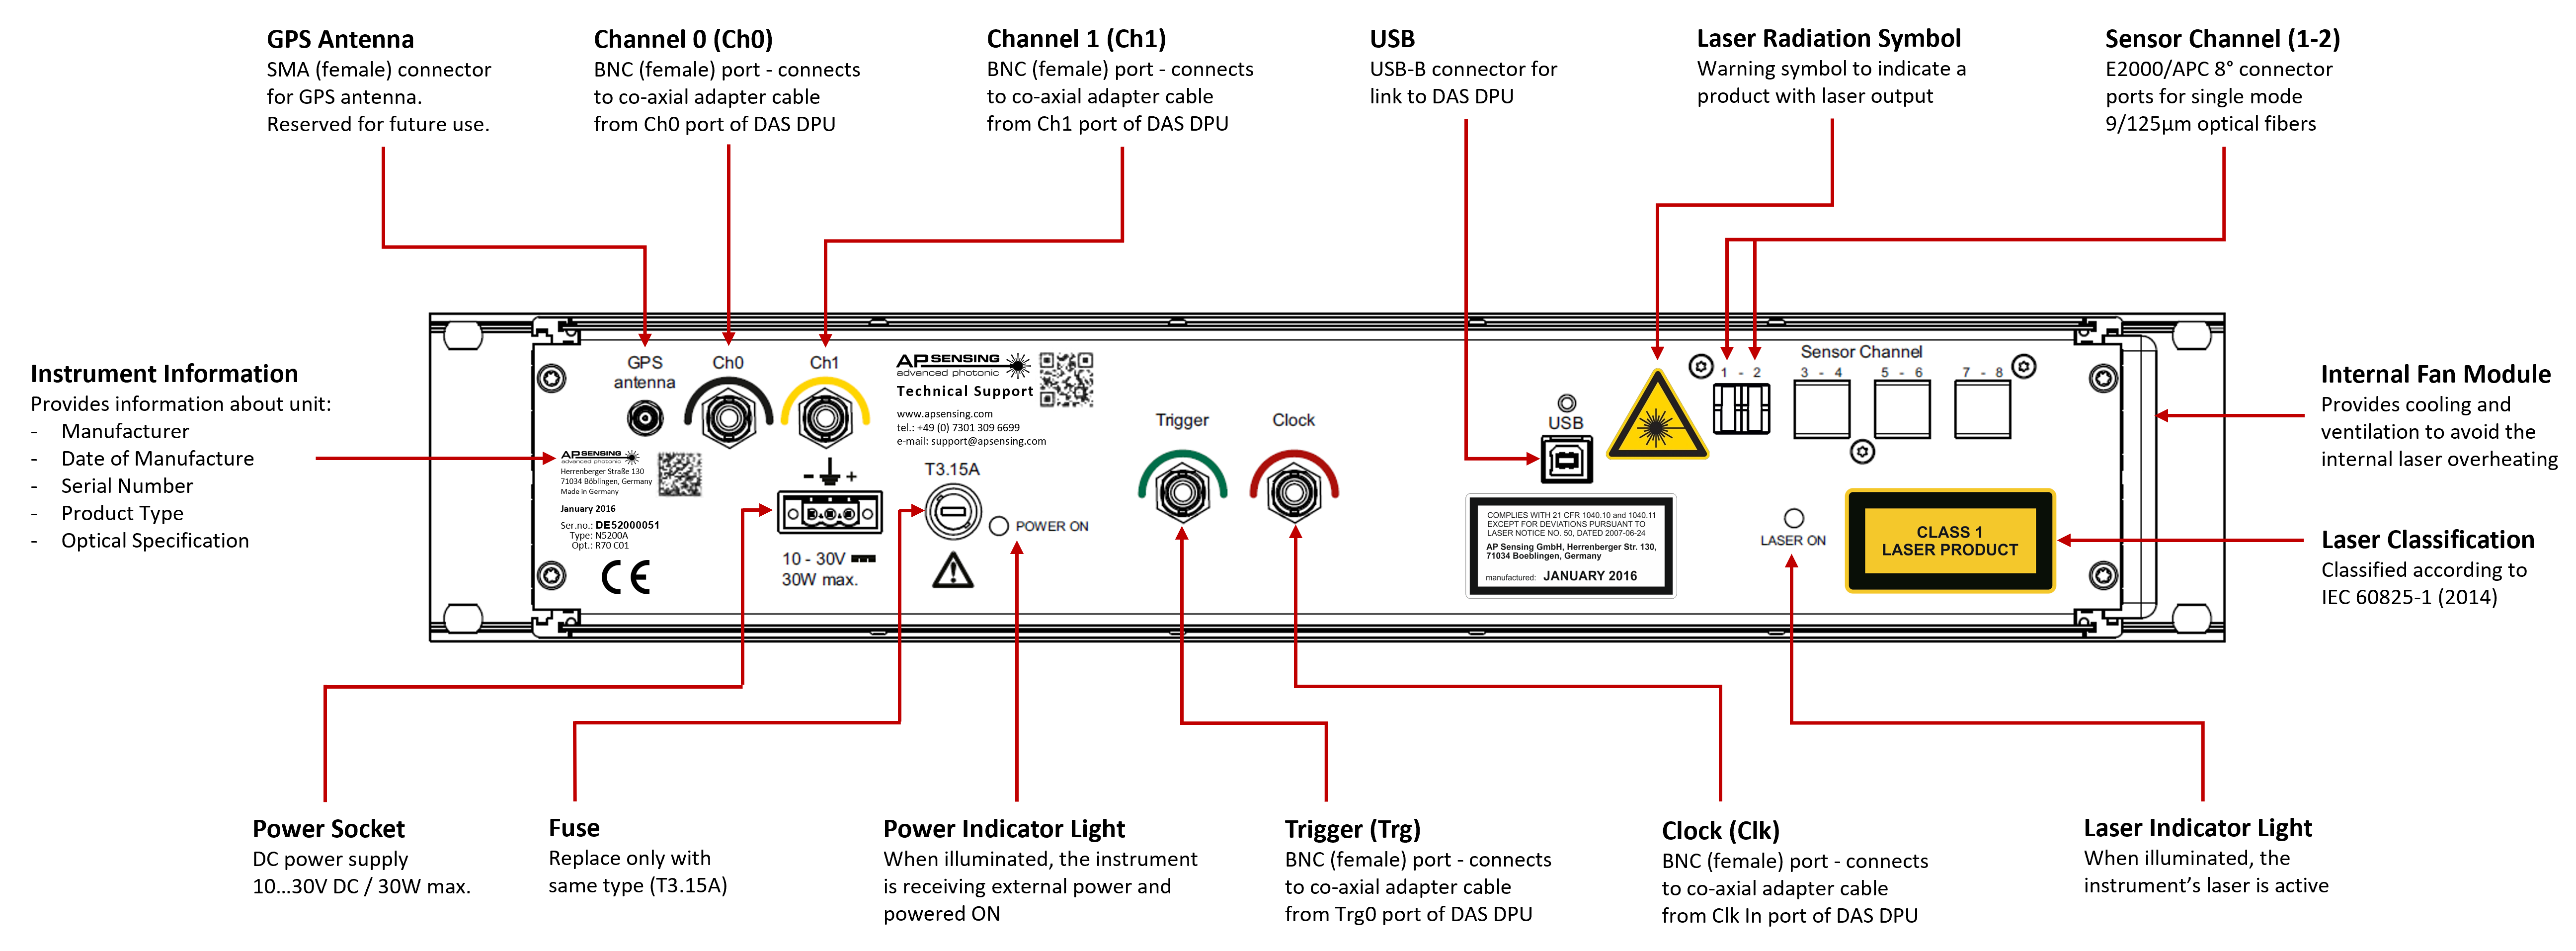
\includegraphics[width=\linewidth]{Bilder/jpg/DAS IU Technical Description.png}
    \caption{DAS IU rear panel view~\cite{DAS_Manual}}
    \label{IU}
\end{figure}

The IU(top) has two channels (horizontal and vertical polarization) which are connected to the DPU(bottom). A USB connector is also connected to the DPU(bottom). A Power socket is needed to power the IU. The trigger which is used to trigger sending of laser pulse is also connected to the DPU. A Digitizer inside the DPU(bottom) is used for synchronization between the IU(top) and DPU(bottom). The IU(top) contains a reference coil of 120m optical fiber inside the case unit. The primary function of this reference coil is to monitor system noise and to checkw whether equipment is measuring accurately. 

\begin{figure}[h]
    \centering
    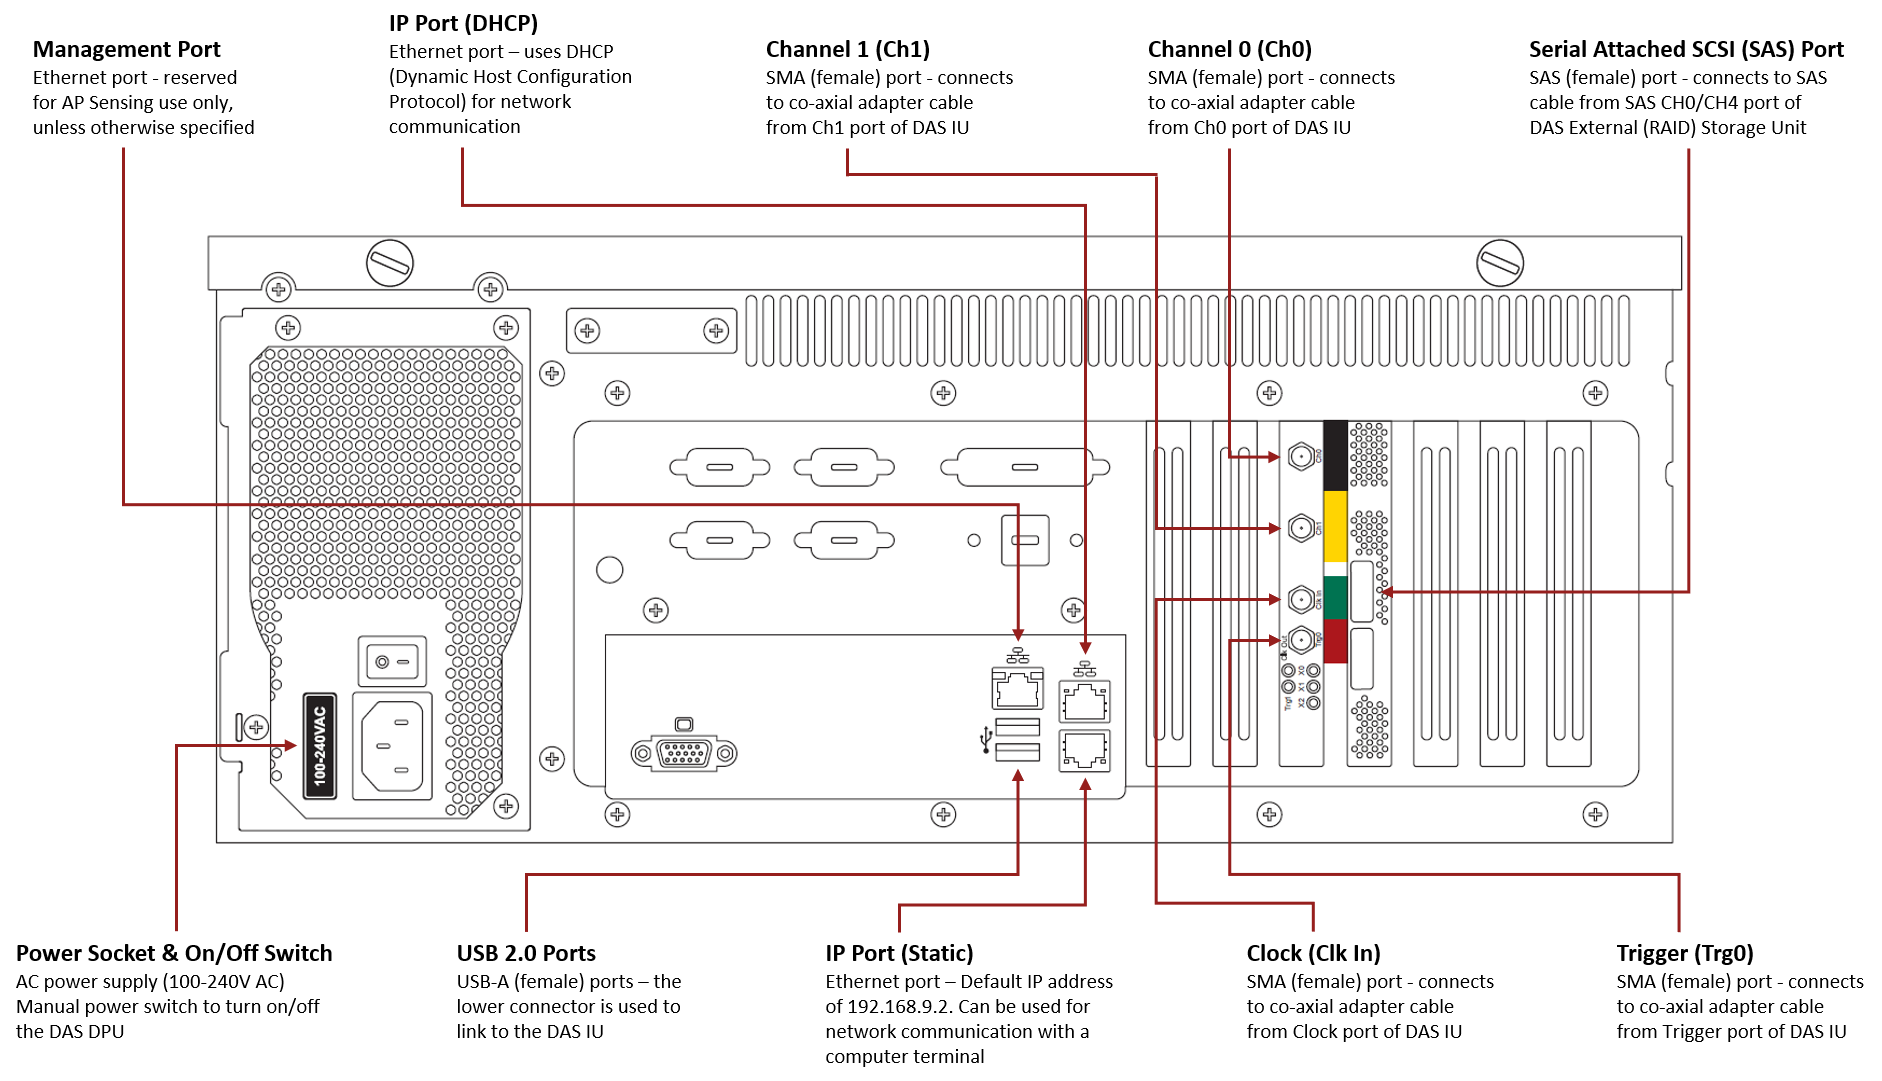
\includegraphics[width=\linewidth]{Bilder/jpg/DAS DPU Rear.png}
    \caption{DAS DPU rear panel view~\cite{DAS_Manual}}
    \label{DPU}
\end{figure}

Figure~\ref{DPU} show the rear view of the DPU of the DAS system. All the connections like the channels, USB, trigger and clock coming from the IU needs to be connected to the DPU. The DPU needs a separate power connection to power it up. There is also an Ethernet port which is used to connect the DAS system to network. The DAS system is connected to a computer via DAS Configurator application if the IP address of the system is known. All the calculations are started through this app. The data is stored in the form of HDF5 file. There are two SSDs available inside the DPU which can be used to store data. The stored data is automatically overwritten once when the capacity limit is reached, following the first-in, first-out (FIFO) approach. There is also other functionality that the data will be erased 30 days after the data is being stored. 

The data outputted from the DPU is made available in the three different formats. 

\begin{itemize} 
    \item{Phase (Dynamic Strain):} 
    This data type provides the raw signal of dynamic strain along the fiber, making it the most data-intensive of the three.

    \item{FBE (Frequency Band Energy):} 
    This data type aggregates the energy within each defined frequency band. After the backscattered signals are captured at each distance channel, they are divided into separate frequency ranges (e.g., 8-20 Hz). The total energy in each band is then displayed in the waterfall plot in Figure~\ref{DAS_waterfall} of the DAS Configurator Client. Its primary purpose is to differentiate between various acoustic events.

    \item{DTGS (Distributed Temperature Gradient Sensing):} 
    This data type highlights gradual variations in the signal arising from bulk temperature or strain effects. Conceptually, it functions like an additional low-frequency band, as the phase signal is analyzed at frequencies below 0.5 Hz.
\end{itemize}


\subsection{DAS Configurator Client}\label{sec:config_app}
DAS Configurator Application is an easy-to-use graphical interface for AP Sensing DAS systems. It allows users to configure and run measurements on the DAS system. The recording and saving of the measured data is also be done which can be useful for analysis and testing of trained models like ConvNext V2 and EfficientNet. It also helps in analyzing and visualization of the data. The data is collected from the DPU which acts as a server. It is designed to continuously run to record the data. The DAS client configurator application is installed on a separate computer which is connected to the DAS DPU via Ethernet. 

\begin{figure}[h]
    \centering
    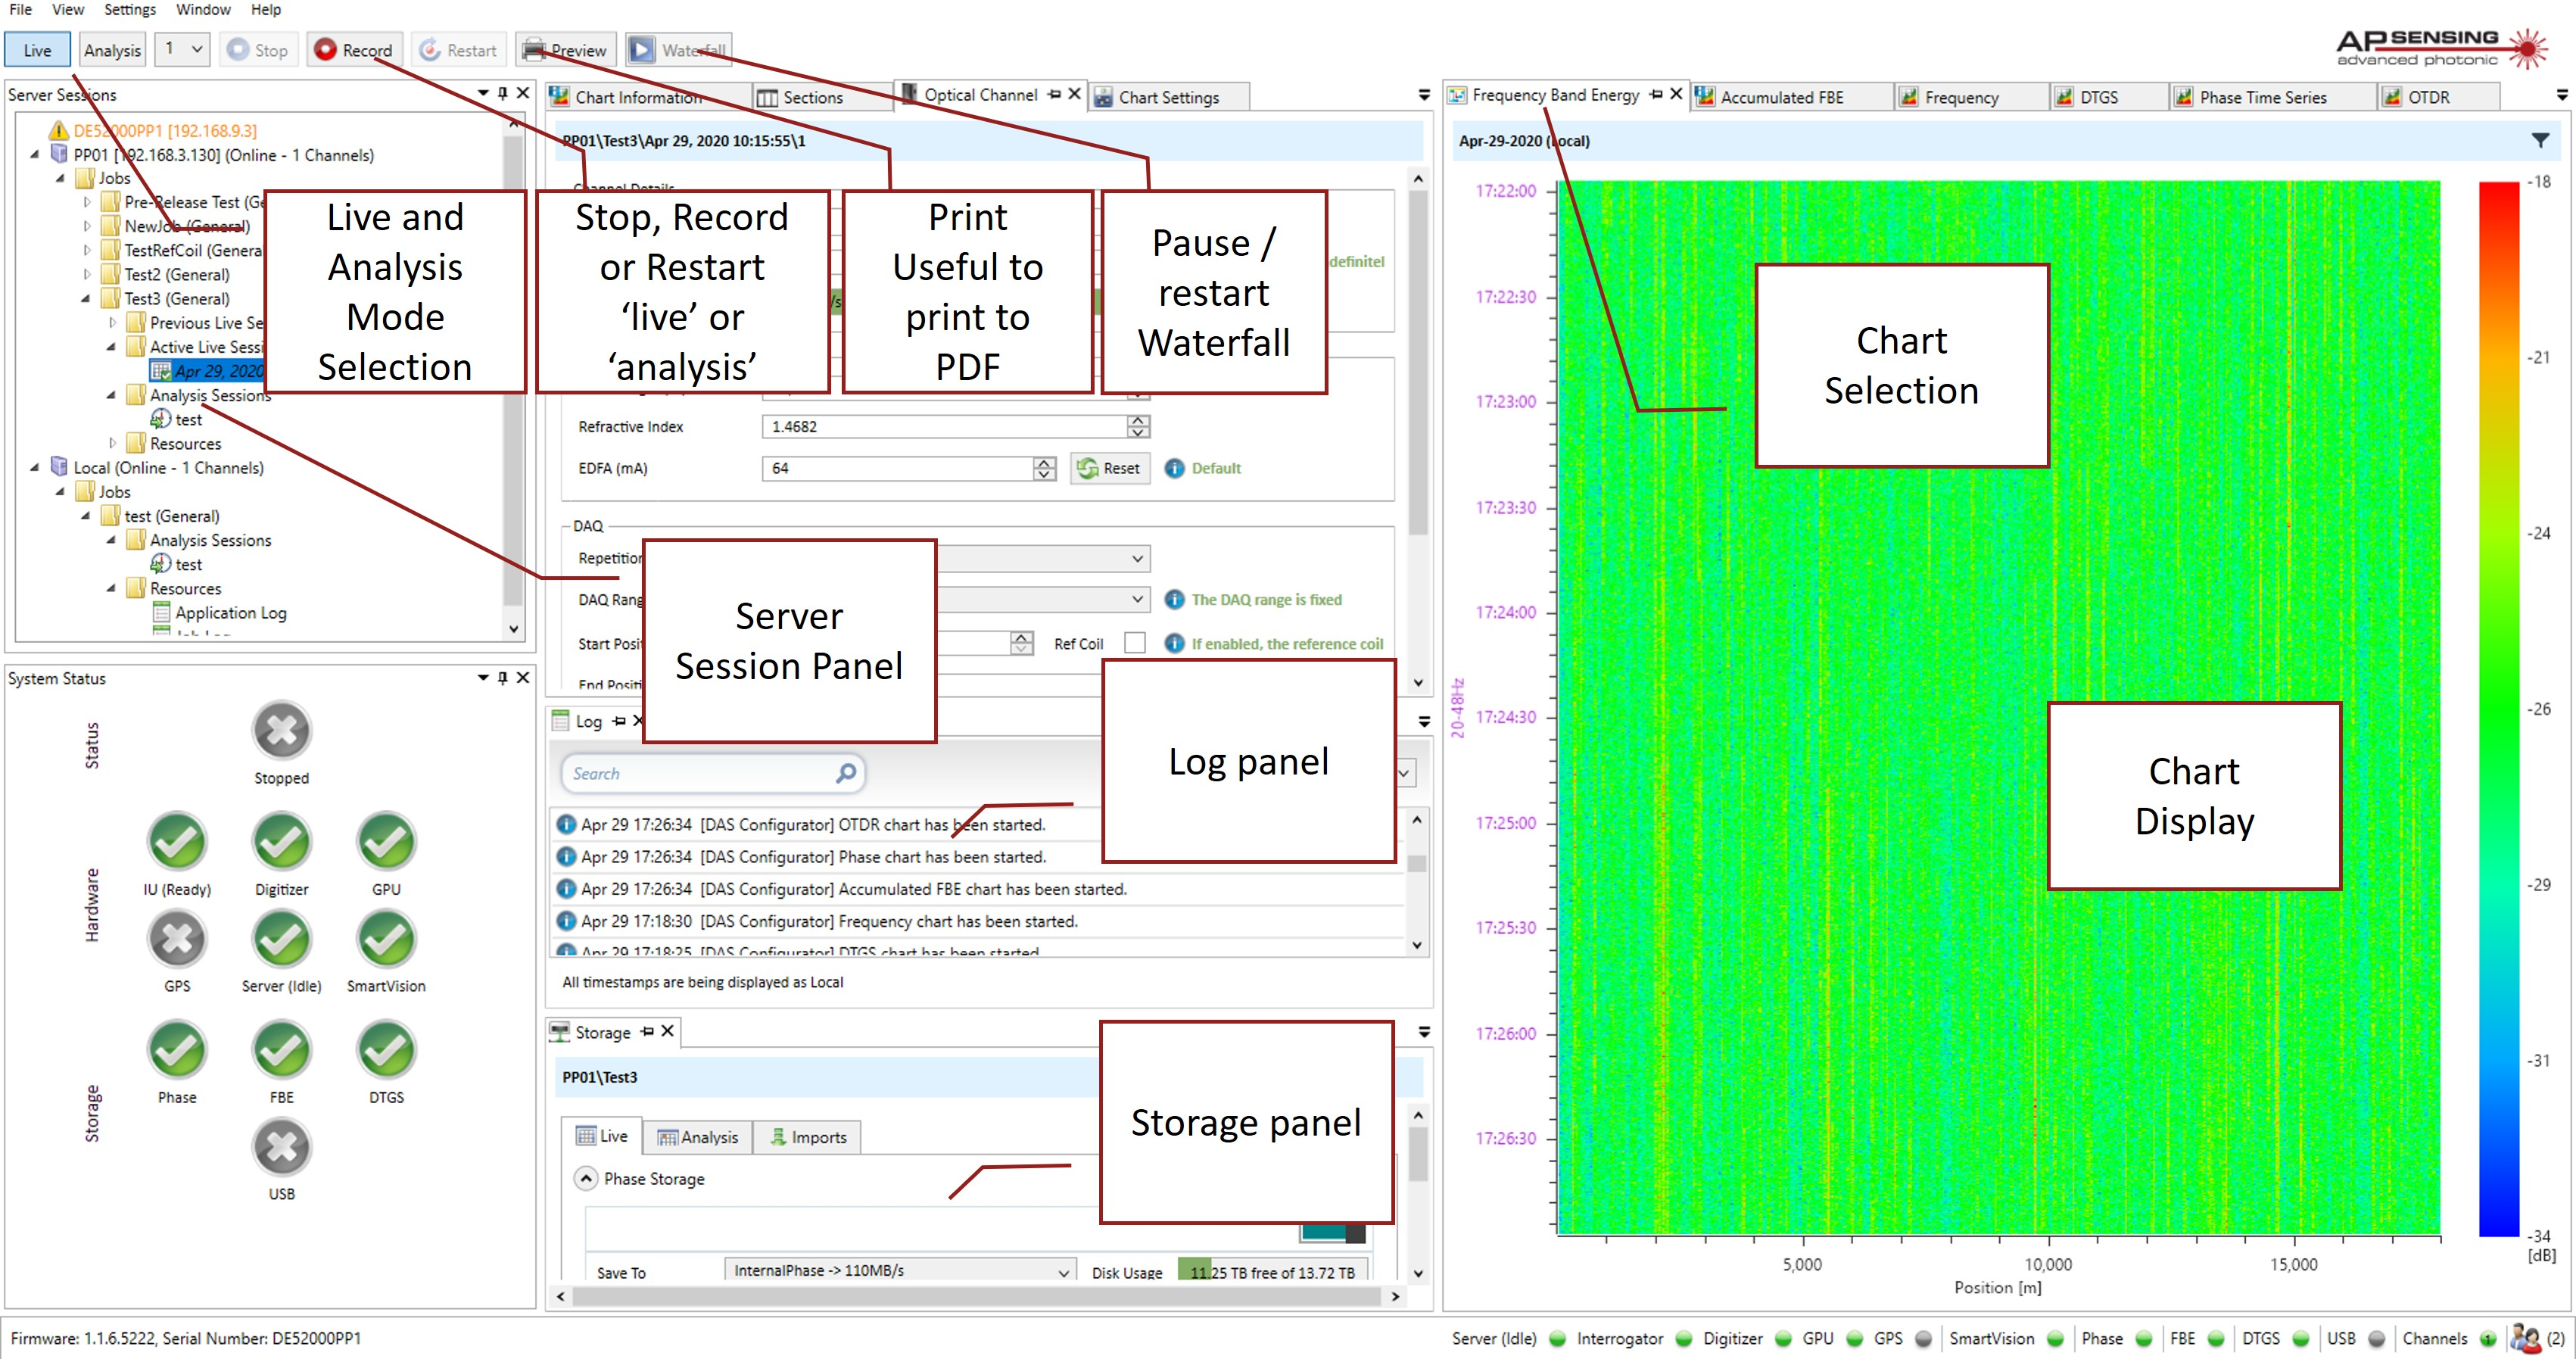
\includegraphics[width=\linewidth]{Bilder/jpg/DAS_config.jpg}
    \caption{Graphical Interface of DAS Configurator Application~\cite{DAS_Configurator_Manual}}
    \label{config}
\end{figure}

Figure~\ref{config} shows the graphical interface of the DAS Configurator Application. The top and bottom bars are fixed while all other charts and panels are easily configurable. They can be freely enabled or disabled. There is a live and analysis mode selection button which can be used to select the respective modes. Then the stop, record or restart button which can be used to the respective tasks with the session. The print button is used to print the screen to a pdf file. The pause/restart button is used to perform the respective operations on the waterfall diagram. Different charts like Phase, FBE and DTGS which can be selected for the layout. The server session panel where different recording session are stored in which all the data related to recording like the time of start and stop of the session, HDF5 files stored can be accessed. The storage panel  shows the available disk space on the drive. The log panel is used to keep the log of the events which happen during the entire session. 

\begin{figure}[h]
    \centering
    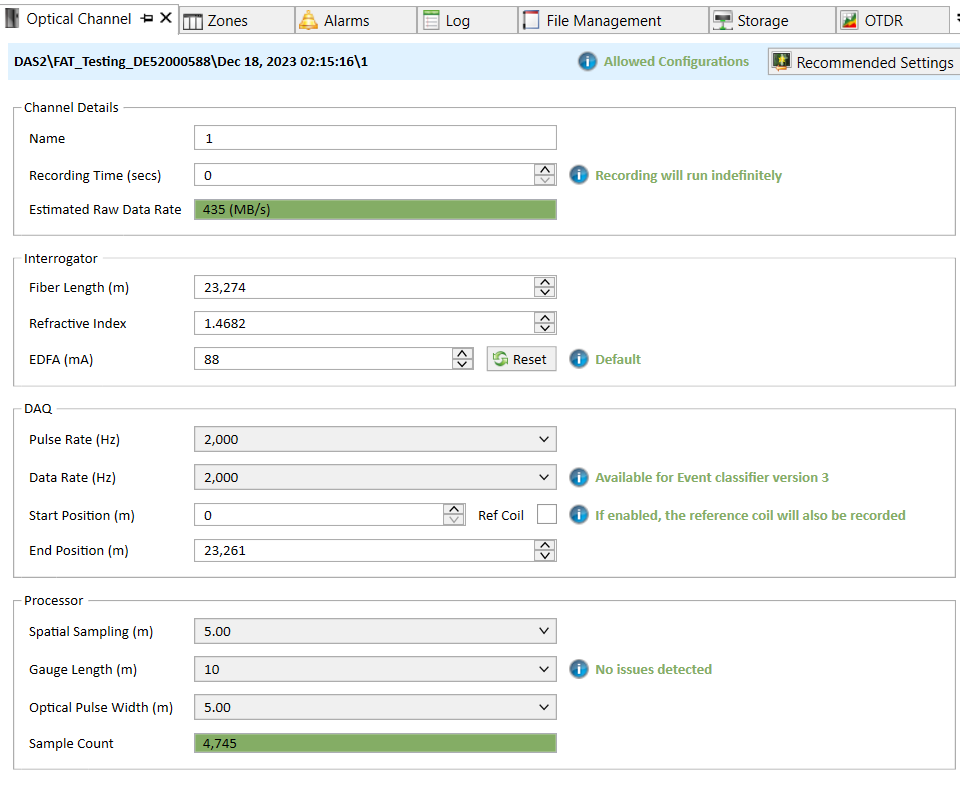
\includegraphics[width=0.8\linewidth]{Bilder/jpg/optical_channel.png}
    \caption{Optical Channel Window in DAS Configurator Application}
    \label{optical}
\end{figure}

Figure~\ref{optical} gives an overview of the optical channel settings that needs to be done on the DAS system. All the configuration settings for the session are done here. The system specifies the channel's name using the "name" field, and it defines the recording time as the duration (in seconds) for which the recording is performed. The maximum data is 960MB/s and if the date rate is exceeded the field turns orange and a warning message is displayed or else its green. Fiber length is actual length of the cable. Refractive index is 1.4682 which is the default value for the single mode fiber. The value can be changed if the manufacturers value of the fiber is different. EDFA value is to be kept unchanged and is adjusted by the production team at AP Sensing. Pulse rate is the laser pulse rate of the DAS interrogator and maximum rate can be given by (math equation). Data rate is the rate of output traces per second, which can be lower than Pulse Rate to allow oversampling. The start and end position are the positions of start and end point of the recording respectively. The spatial sampling is sampling rate along the fiber length and can be adjusted from 1.25m to 40m. Gauge length is the distance between two phase measurements, determining spatial resolution and can be in the range 3.75m to 80m. Optical pulse width is the actual physical width of the pulse, adjustable by trained user which affects the DAS performance. The sample count are the number of samples to be processed. These are the total points in the fiber that are responsible for collecting the data which then further used for plotting the waterfall diagram or stored in HDF5 format. User can select which data can select the format of data (Phase, FBE or DTGS) as explained in previous section. The data from HDF5 files can be retrieved using any programming language as there are already packages or libraries available which can be used to access them. 

\section{Image Recognition using Machine Learning}
Image Recognition is a process of detecting different patterns in the images and detecting similar images. Image Recognition is useful in crucial applications like autonomous vehicles, medical diagnosis and visual search. It has been revolutionized by deep learning techniques such as convolutional neural networks (CNNs) and recurrent neural networks (RNNs) as it has better performance for image recognition. Machine learning methods for image recognition rely on algorithms trained on extensive collection of images. These systems automatically detect patterns and visual elements(edges, textures and colors) critical for categorization. After the training phase where the model is trained on a particular set of images, the model can automatically detect similar sort of patterns and images thus enabling accurate and scalable image analysis~\cite{chandni}. 

For a model to detect the similar sort of patterns, it needs to be trained and evaluated on a dataset. The dataset needs to be collected where the different kind of images need to be labelled and based on these labels the model is trained. Different augmentation techniques are also applied to the training dataset such as flipping images or rotation. The model training is thus generalized and is able to detect the images correctly irrespective of what new images the model comes across. The model should be trained in such a way that it doesn't memorize the patterns in images but actually learns the patterns and generalize them properly. Evaluation of the model needs to be done on the entirely different dataset which is not used in training phase. The performance of the model is determined by how well it performs on the evaluation dataset.

\begin{itemize} 
    \item \textbf{Data Preparation:} 
    Preparing training and testing data by gathering the different kind of images on which the model needs to be trained. The preprocessing steps need to be applied on the images in Figure~\ref{sec:preprocessing}. These help in consistency of the data and help in proper visualization of the images.

    \item \textbf{Finding a model:} 
    The pre-trained models are the models which are trained on the image dataset available online. These models are trained on large datasets and are available for use. The models can be used as a starting point for the training. The model can be trained on the dataset available and then fine-tuned to get the best performance. The models can be used as a black box where the model is trained on the dataset and then used for evaluation. 

    \item \textbf{Train the Model:} 
    Training a model requires to provide a model with training data. Training data can be any form of images which are given to the model. Images are passed through various layers of the model from which understands the patterns. Model goes through this training data several times, the model will automatically determine the most crucial aspects. Model will acquire the ability to detect more characteristics and distinguish between various classes of data.

    \item \textbf{Evaluation Data:}
    To check whether the model is trained properly or not, the model needs to be evaluated on a different dataset which is not used in training phase. Evaluation dataset should be similar to the training dataset but should not contain any of the images from the training dataset. Evaluation dataset is used to check how well the model is trained and how well it can detect the patterns in the images. The performance of the model is determined using the confusion matrix. Confusion matrix is a table which shows the actual and predicted values of the model. Confusion matrix is used to check how well the model is trained and how well it can detect the patterns in the images. 
\end{itemize}

\subsection{PyTorch}\label{sec:PyTorch}
PyTorch~\cite{PyTorch_website} is a machine learning library that provides an imperative and Pythonic coding style, emphasizing ease of use, seamless debugging, and alignment with other scientific computing libraries, while maintaining efficiency and supporting hardware accelerators like GPUs. The trend started in domain specific languages such as APL, MATLAB, R which turned multidimensional arrays (also known as tensors) into objects supported by mathematical primitives to manipulate them. Other libraries such as NumPy, Torch, Eigen and Lush made array-based(tensor) programming productive in general purpose languages such as Python and C++~\cite{pytorch}. 

Deep learning is computations on tensors, which are generalizations of a matrix that can be indexed in more than 2D. Data required is extracted in the form of NumPy arrays. Arrays are preprocessed according to the requirement in such a way that patterns in the images are clearly visible. Then NumPy data is converted into a tensor which then feed to a model for training. The model trains based on this tensor. There are various metrics which need to be monitored while training the model to see if the model is learning efficiently and not memorizing the patterns. 

The efficacy of the model is the ability of a model to make the correct predictions. There are various metrics like Accuracy, Precision and Recall which need to be considered and are important to understand how well the model is trained. It revolves around categorizing the data points into predefined classes which is also known as classification problems. For instance, determining whether an email is a spam or not can be treated as an example of a binary classification. As the complexity of the model increases and the number of classes increase the intricacy of model increases. These metrics need to be monitored not only for the overall model but also over each class to see how well the model is classifying~\cite{Efficacy}. 

\subsubsection{Confusion Matrix}
The confusion matrix is a very important element in evaluating how well the model is trained. Model is improved by monitoring these metrics. The table~\ref{tab:confusion_matrix} shows the different metrics. The comparison of actual outcomes with predicted outcomes is done. The class imbalance is understood here and based on that it is determined whether the problem is with a specific class or the whole model. 

\begin{table}[ht]
    \centering
    \begin{tabular}{l|c|c|c}
      \toprule
      & \multicolumn{2}{c}{\textbf{Predicted}} & \\
      \cmidrule(lr){2-3}
      & \textbf{Positive} & \textbf{Negative} & \textbf{Total} \\
      \midrule
      \textbf{Actual} \tabularnewline
      \textbf{Positive} & True Positive (TP) & False Negative (FN) & Total Positive \\
      \midrule
      \textbf{Negative} & False Positive (FP) & True Negative (TN) & Total Negative \\
      \midrule
      \textbf{Total} & Total Predicted Positive & Total Predicted Negative & Total Samples \\
      \bottomrule
    \end{tabular}
    \caption{Confusion Matrix Example}
    \label{tab:confusion_matrix}
  \end{table}

  The four main elements can be explained as follows which will give an overview of the models expected and actual outputs.
  \begin{itemize}
    \item \textbf{True Positive (TP)}:  The model correctly identifies instances belonging to the positive class. \\
      \textit{Example}: Spam emails automatically routed to the spam folder.

      \item \textbf{True Negative (TN)}: The model accurately identifies instances belonging to the negative class \\
      \textit{Example}: Important emails delivered directly to the inbox.
  
        \item \textbf{False Positive (FP)}: The model incorrectly classifies negative instances as positive (Type I error).
      \textit{Example}: Important emails mistakenly sent to the spam folder.
  
    \item \textbf{False Negative (FN)}:The model fails to identify positive instances, classifying them as negative (Type II error). \\
      \textit{Example}: Spam emails slipping through the filter and appearing in the inbox.
  
  \end{itemize}

  There are different metrics like accuracy, precision and recall which can be calculated using the elements from the table~\ref{tab:confusion_matrix}. Ideally all the values should be high but depending on the use case the values are traded off to give the best performance for the case. Accuracy can be misleading as it fails to measure overall correctness when classes are imbalanced. So precision or recall need to be used to identify the performance of the minority class. The spam email detection example will give the better understanding for the same. The model labels all email not spam would get 95\% accuracy but fails to detect any spam. If the model detects 80\% of spam emails(high recall) but mislabels 20\% of the legitimate emails(low precision) user can get annoyed by false alarms. 

  \subsubsection{Accuracy}
  Accuracy is a metric that quantifies the overall performance of a classification model by measuring the proportion of correctly predicted instances (both true positives and true negatives) relative to the total number of instances. It is calculated using the formula:

  \begin{equation}
    \text{Accuracy} = \frac{TP + TN}{TP + TN + FP + FN} \times 100\%
    \label{eq:accuracy}
  \end{equation}
  where:
  \begin{itemize}
    \item $TP$ = True Positives
    \item $TN$ = True Negatives
    \item $FP$ = False Positives
    \item $FN$ = False Negatives
  \end{itemize}

  Accuracy is often the first metric evaluated for classification tasks due to its simplicity and intuitive interpretation as a percentage of correct predictions. It works well when the dataset has balanced class distributions. However in imbalanced scenarios other metrics also need to be considered. In real life scenarios the cost of false negative (failing to identify a disease) might be more severe than a false positive in a medical diagnosis.

  \subsubsection{Precision}
  Precision is a metric providing how well the model predicts positive instances while minimizing the risk of false alarms. Precision is an important metric in classification problems where the cost is high for false positives. Precision is true positives from all positives detected by the model. The precision of a classification model is calculated as:

  \begin{equation}
    \text{Precision} = \frac{TP}{TP + FP} \times 100\%
    \label{eq:precision}
  \end{equation}
  where:
  \begin{itemize}
    \item $TP$ = True Positives
    \item $FP$ = False Positives
  \end{itemize}

  Precision is very important when false positives are costly. False positives are very costly in instances like fraud detection systems, where flagging legitimate transactions leads to unnecessary investigation and customer dissatisfaction, potentially causing business loss. Precision only focuses on positive cases, neglecting all negative cases. A model achieves high precision by making fewer positive predictions, resulting in missing many positive cases.

\subsubsection{Recall}
Recall is a metric representing the proportion of actual positive cases identified by the model. Recall is also known as sensitivity or the true positive rate. The recall of a classification model is calculated as:

\begin{equation}
  \text{Recall} = \frac{TP}{TP + FN} \times 100\%
  \label{eq:recall}
\end{equation}
where:
\begin{itemize}
  \item $TP$ = True Positives
  \item $FN$ = False Negatives
\end{itemize}

Recall is important where false negatives are costly. Recall focuses on finding all positive cases even with more false positives. A model may predict most instances as positive to achieve high recall. This leads to many incorrect positive predictions. Using these metrics and making adjustments as needed, the model is trained according to requirements. 

\subsection{Data Augmentations}\label{sec:augmentation}
Data augmentation implies a collection of different techniques  to enhance the diversity and volume of training datasets to improve the model performance. The techniques include geometric transformations, color space adjustments, filter-based adjustments, filter-based methods, image mixing, random erasing. This helps in improving model generalization and diversifying the dataset thus helping in dealing with overfitting problem~\cite{Augmentation}. 

The data augmentation helps in generalizing the data better which will help in training the model with the patterns instead of model memorizing the images. Model will perform better on the unseen data when augmentation techniques are used. 

\subsubsection{Horizontal Flipping}
Horizontal flipping mirrors the image along the vertical axis, thus creating a horizontally reversed image. This helps model to generalize better thus reducing the overfitting. Figure~\ref{hflip} shows the horizontal flip of cat image.

\begin{figure}[h]
    \centering
    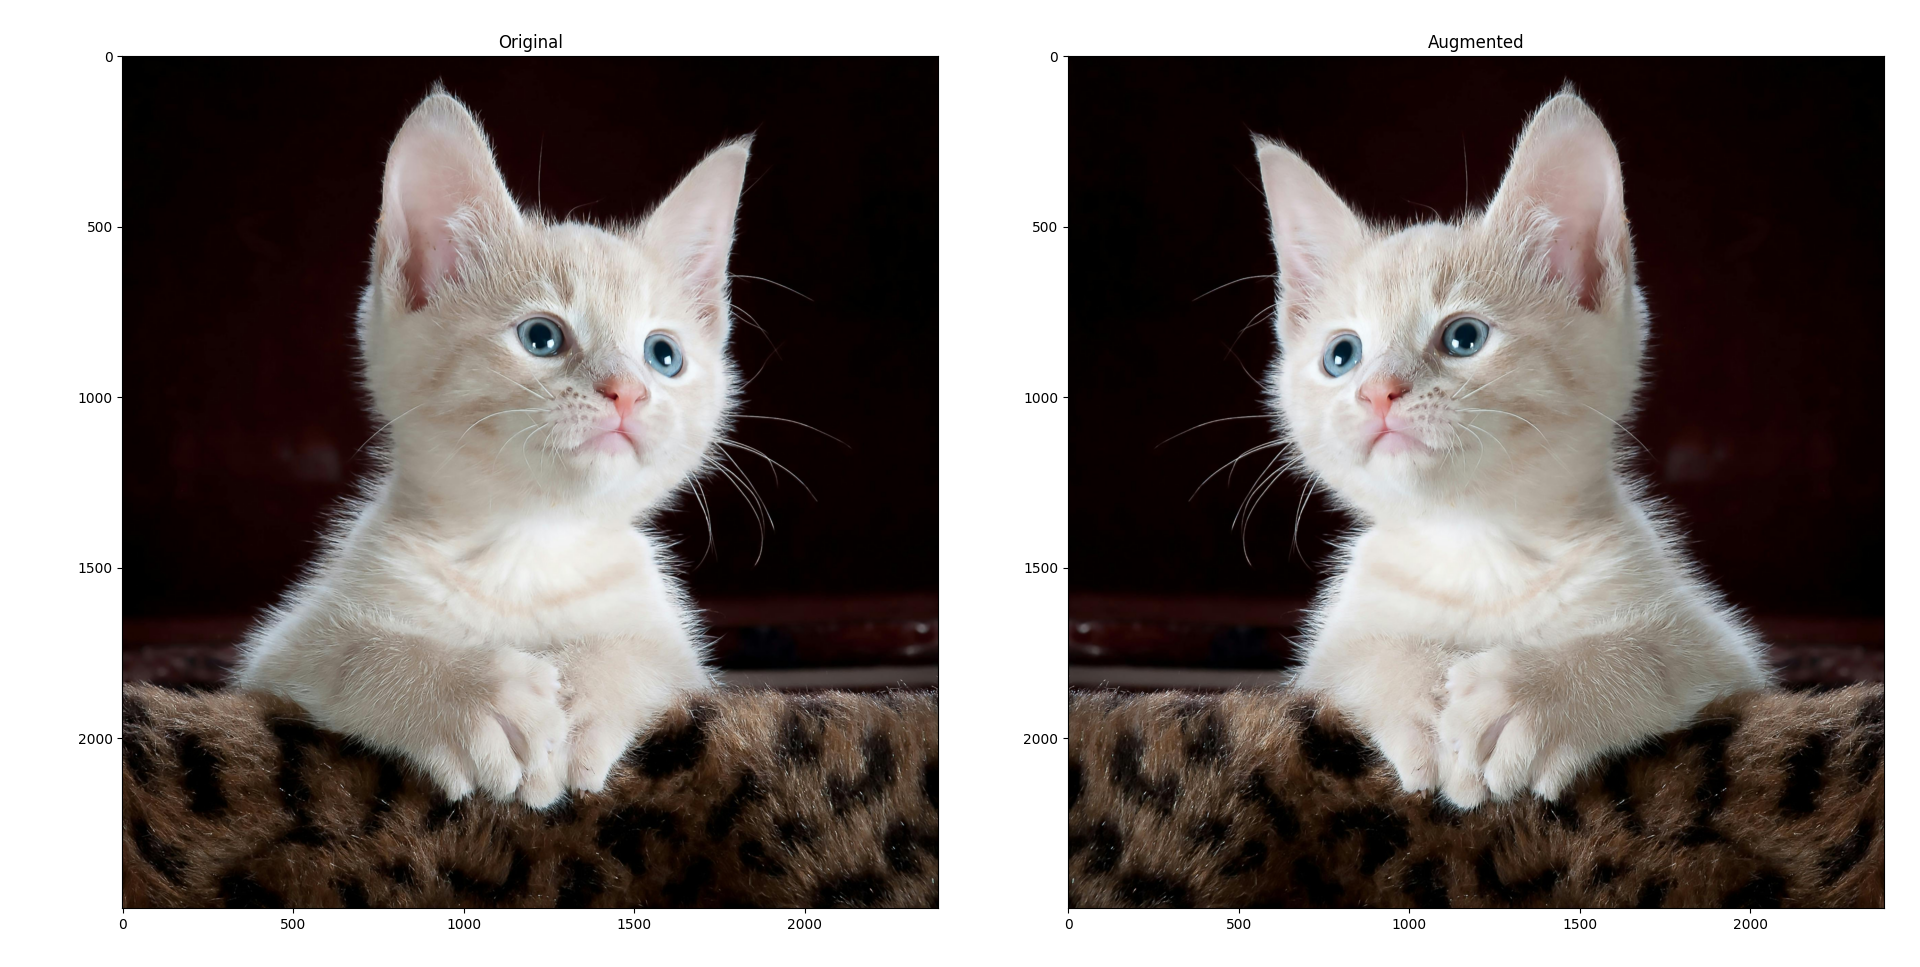
\includegraphics[width=0.6\linewidth]{Bilder/jpg/Horizontal flip.png}
    \caption{Horizontal Flip~\cite{kitten}}
    \label{hflip}
\end{figure}

\subsubsection{Vertical Scaling}
Vertical scaling or amplitude scales the image on the vertical or amplitude scale, thus creating image which is stretched along the vertical or amplitude axis. This also helps in generalization and detects images which are stretched on the vertical scale. Figure~\ref{amp} shows it with cat image how the image is stretched along the vertical scale or amplitude scale .

\begin{figure}[h]
    \centering
    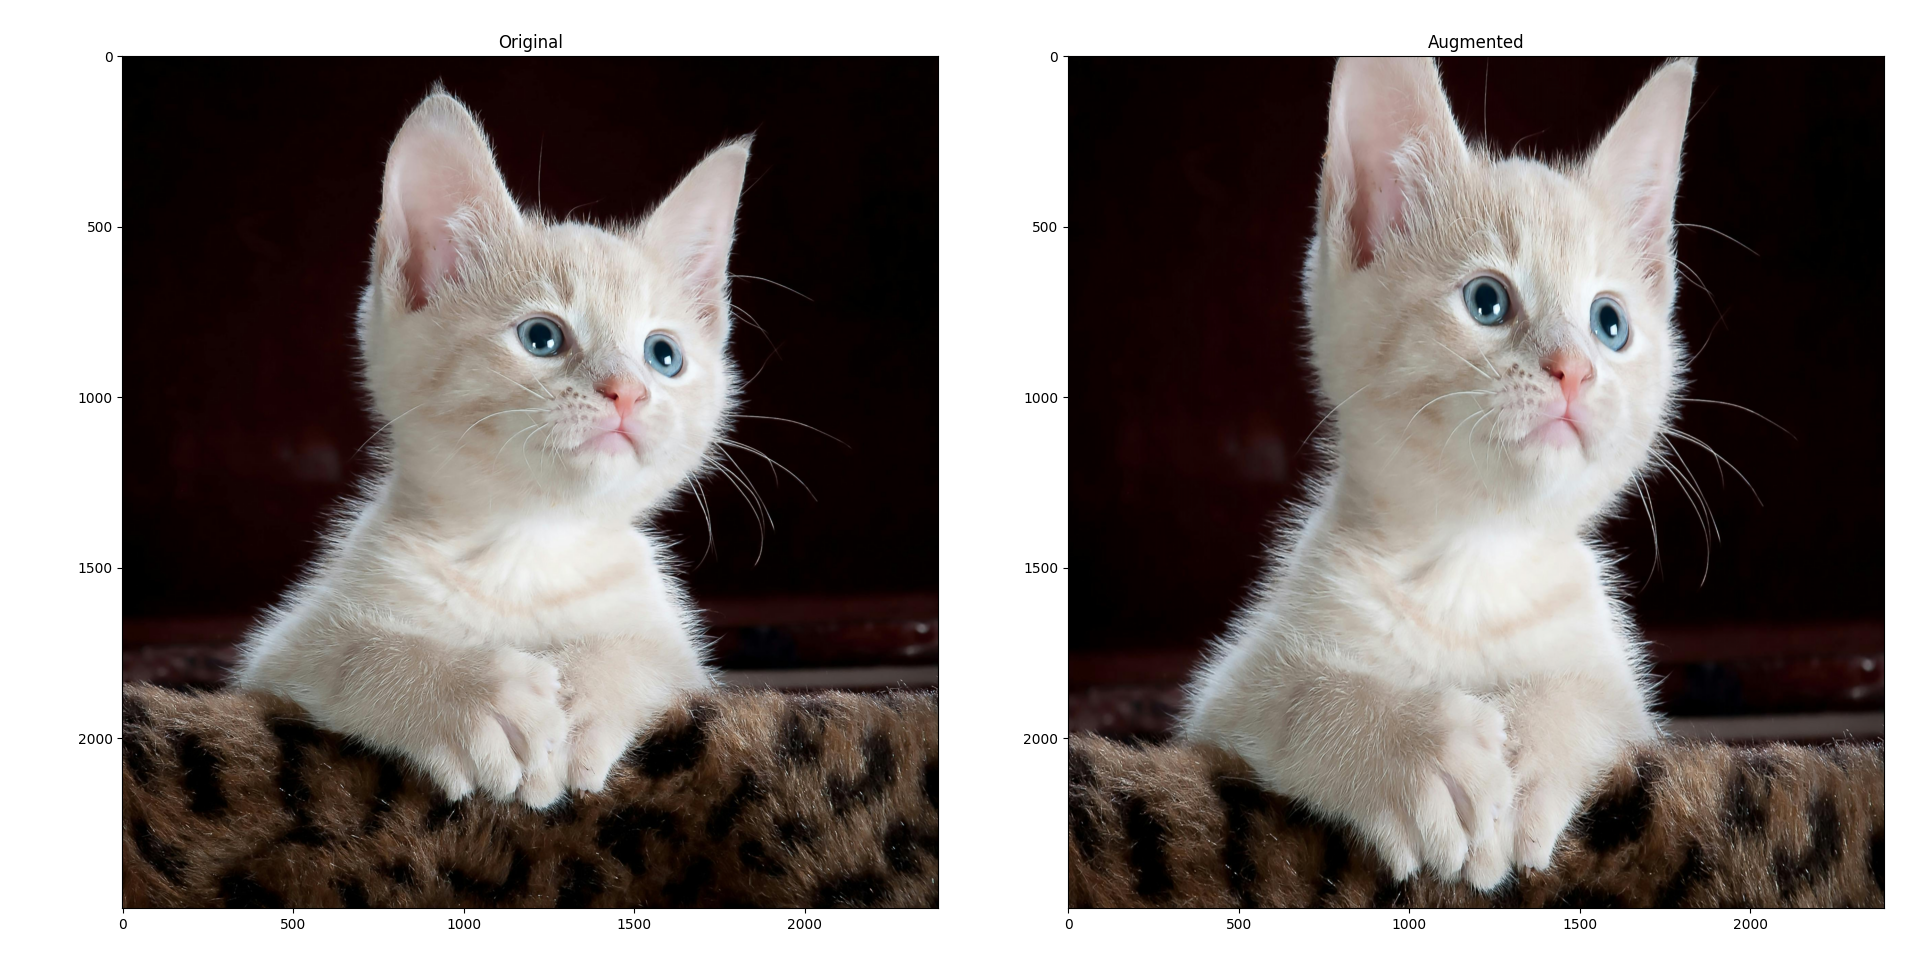
\includegraphics[width=0.6\linewidth]{Bilder/jpg/amp.png}
    \caption{Vertical Scaling~\cite{kitten}}
    \label{amp}
\end{figure}

\subsubsection{Horizontal Scaling}
Horizontal scaling or time scaling is amplifying the image across the time scale or horizontal scale , thus creating image which is stretched across the time or horizontal axis. This also helps in generalization and even if the images which are stretched on horizontal scale. Figure~\ref{time} shows this with a cat image where it is stretched along the time scale or horizontal scale for. 

\begin{figure}[h]
    \centering
    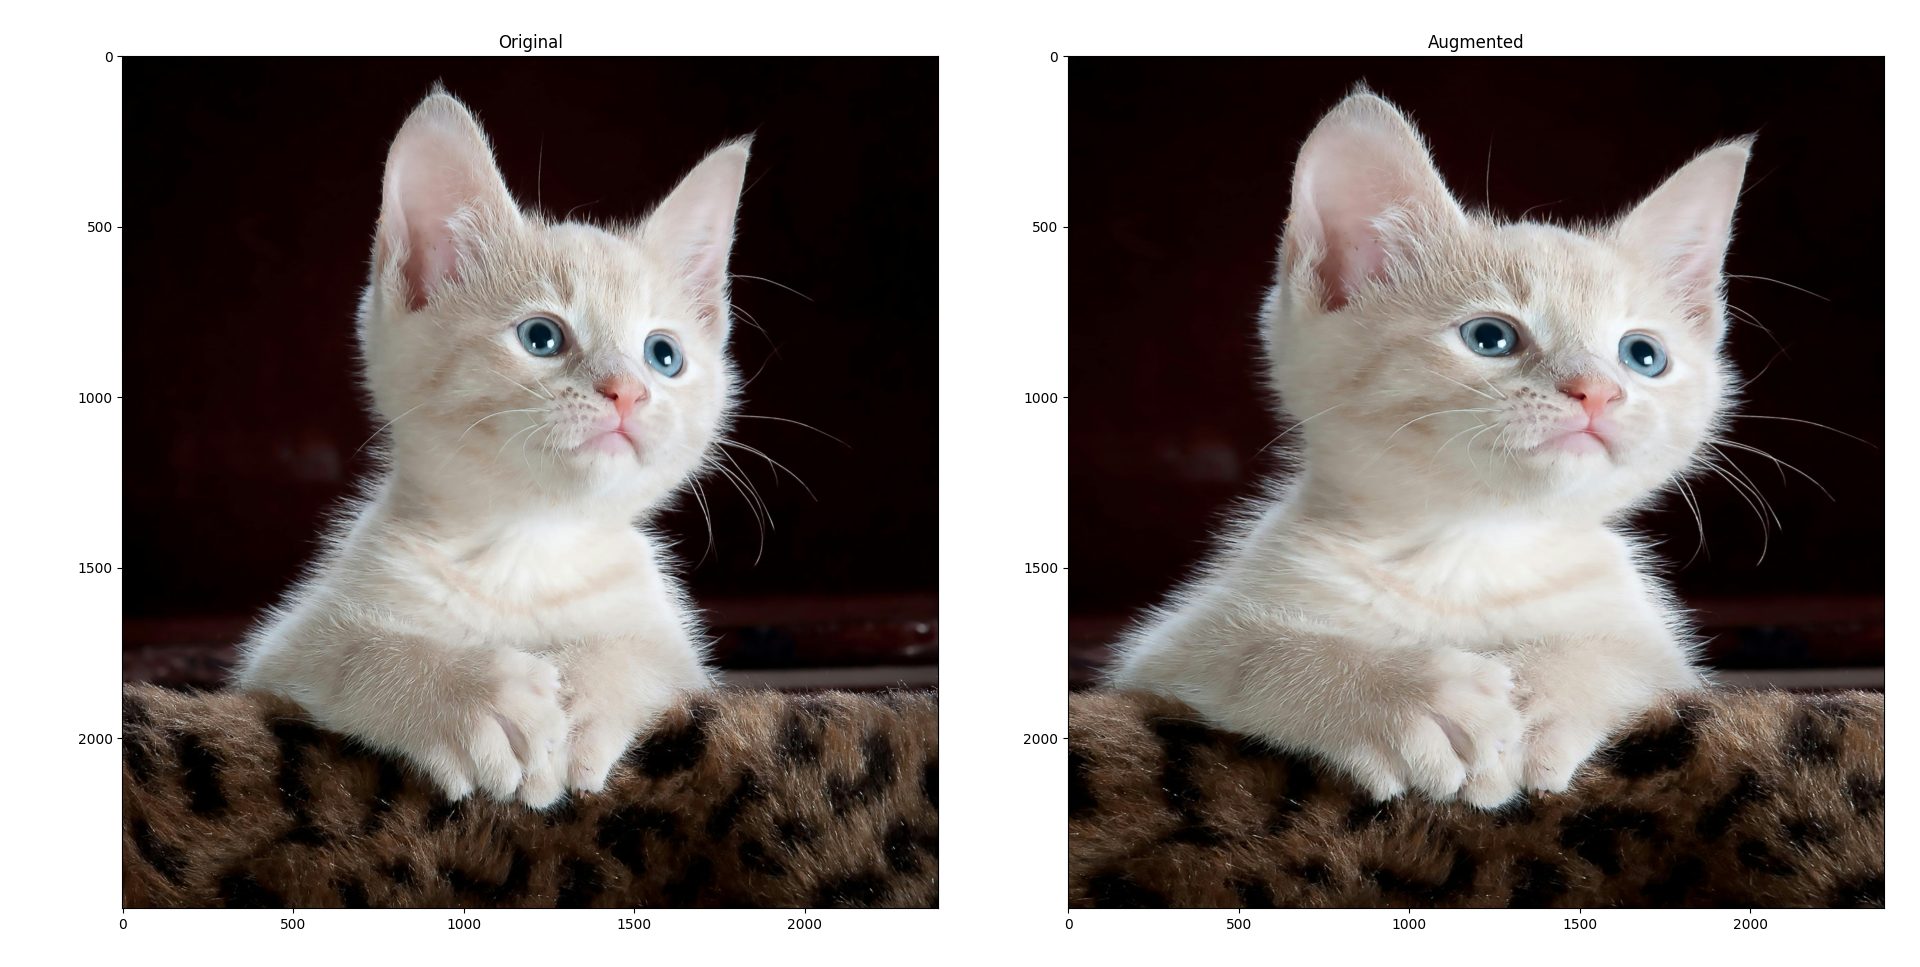
\includegraphics[width=0.6\linewidth]{Bilder/jpg/affine.png}
    \caption{Horizontal Scaling~\cite{kitten}}
    \label{time}
\end{figure}

\subsubsection{Gaussian Noise Injection}
In this augmentation, gaussian noise is injected into the image to increase the robustness and generalization of the model. The noise is added to the image by controlling the mean and standard deviation. Figure~\ref{noise} demonstrates injecting the noise to a cat image with standard deviation set to 0.6 for demonstration purposes so that injection is visible.

\begin{figure}[h]
  \centering
  \includegraphics[width=0.6\linewidth]{Bilder/jpg/Noise.png}
  \caption{Gaussian Noise Injection~\cite{kitten}}
  \label{noise}
\end{figure}

\subsection{Kornia}

Kornia is an open-source computer vision library built on top of PyTorch\ref{sec:PyTorch} that provides a familiar, NumPy-like API for classical vision operations (e.g.\ geometric transforms, filtering, feature detection) in a fully differentiable and GPU-accelerated form. Unlike the traditional 'torchvision.transforms'~\cite{torchvision2024}, which execute many augmentations on the CPU and then copy results to the GPU, Kornia implements each operation as a native PyTorch module or function that runs directly on CUDA. This tight integration allows to include data augmentations as part of the model's computation graph-making them differentiable, reducing host-device synchronization overhead, and enabling end-to-end optimization when desired.

In our spectrogram-based footstep classification pipeline, we use several Kornia augmentations (Horizontal Flip, Normalize) alongside custom PyTorch modules.  By leveraging Kornia, we gain:

\begin{itemize}
  \item \textbf{Performance}: All transformations (flips, normalizations, warps) execute directly on the GPU, avoiding costly host-device transfers (i.e., data is not sent back to the CPU for processing) and achieving higher throughput during training.
  \item \textbf{Differentiability}: Since each augmentation is a PyTorch module, gradients can flow through the transform when performing adversarial or meta-learning experiments that require backpropagation through data augmentation.
  \item \textbf{Composability}: Kornia's ops follow the same 'torch.nn.Module' and functional API conventions as PyTorch, allowing seamless integration into 'torchvision.transforms.Compose', 'torch.nn.Sequential', or custom training loops.
\end{itemize}

Together, these features make Kornia an ideal choice for high-performance, flexible data augmentation in end-to-end deep-learning pipelines~\cite{kornia}. 

\section{Literature Review}
DAS has emerged as a versatile tool in detection of various human activities, including footsteps by sensing the ground vibrations. Over the past decade, researchers have explored signal processing, Machine learning (ML), and environmental adaptions to enhance the detection accuracy. This section gives an overview of different studies which shows key advancements and challenges.

\paragraph{Time-frequency preprocessing.}
A crucial first step is turning raw DAS phase traces into a time-frequency representation that makes footsteps stand out. Ekimov and Sabatier~\cite{ekimov2007ultrasonic} showed that human footsteps produce strong components in the 1-4~Hz band (with measurable energy up to 600~Hz outdoors) and used short-time Fourier transforms (STFTs) and spectrograms to isolate these bands. Likewise, K \textit{et al.}~\cite{ks2021acoustic} created synthetic datasets by slicing DAS recordings into 2~s windows and converting them into spectrograms-an approach we adopt directly, since it balances temporal resolution with computational cost.

\paragraph{Deep-learning classification.}
Once a spectrogram is in hand, convolutional neural networks (CNNs) have become the workhorse. Jakkampudi \textit{et al.}~\cite{footstep} applied a CNN to 5~km of outdoor DAS data (2~m channel spacing) and reported 84\% footstep vs background accuracy. To handle overlapping footsteps and changing directions, hybrid ConvLSTM architectures~\cite{zhou2024large} have been proposed improving indoor tracking accuracy to about 81.5\%. In our thesis, we build on these successes by comparing two state of the art backbones (ConvNeXt V2 and EfficientNet) and by introducing a targeted augmentation strategy to further reduce false negatives in challenging overlap scenarios.

\paragraph{Environment and noise adaptation.}
Outdoor DAS must contend with wind and distant traffic noise, while indoor signals suffer multipath reflections. Ekimov~\cite{ekimov2007ultrasonic} emphasized that vibration energy above 600~Hz decays rapidly outdoors, which motivates our choice of filter bank design. Bublin~\cite{bublin2021event} showed that combining DAS with auxiliary sensors (e.g.\ accelerometers) can improve robustness to transient events like excavator digging. Although we focus on single-sensor DAS here, our evaluation framework logs false-positive cases for future data-driven noise modeling or multimodal fusion.

\paragraph{Open challenges.}
Most prior work handles a single pedestrian or controlled corridor; detecting multiple simultaneous footsteps remains hard~\cite{footstep}. We likewise observe increasing false positives when multiple subjects share the same fiber segment. To address this, our model training pipeline incorporates random spatial and amplitude perturbations (Section~\ref{sec:augmentation}) to encourage separation of overlapping patterns laying groundwork for multi-person DAS detection in future extensions.

\paragraph{Benchmarking ML on DAS.}
Shi and Zong~\cite{Shi2025Benchmark} present one of the first end-to-end benchmarks comparing classical ML methods (SVM, Random Forest) against modern deep nets (CNNs, Transformers) on real DAS footstep data. They systematically evaluate different spectrogram parameters, data-augmentation recipes, and backbone architectures, and find that a lightweight vision-transformer slightly outperforms CNNs once trained with sufficient augmentation. Their results both validate our choice of ConvNeXt V2 and EfficientNet and underscore the importance of tuning augmentation hyperparameters.

\paragraph{Multimodal contrastive learning.}
Yadav \textit{et al.}~\cite{Yadav2021Contrastive} fuse DAS spectrograms with co-recorded geophone signals in a metric-learning framework. By pulling together matching footstep pairs across sensors and pushing apart non-footstep pairs, they learn a joint embedding that boosts classification accuracy by 15-20 pp over single-sensor baselines. Although our current work is purely DAS-based, their fusion approach offers a clear path to tackle the false-positive challenges we observe when multiple subjects overlap (Section~\ref{sec:augmentation}).

\medskip
By combining the spectrogram windowing strategy of~\cite{ks2021acoustic}, the CNN-based classifiers of~\cite{footstep} and~\cite{zhou2024large}, the rigorous benchmarking from~\cite{Shi2025Benchmark}, and the multimodal fusion ideas of~\cite{Yadav2021Contrastive}, this thesis delivers a robust, end-to-end footstep detector on both single- and ten-channel DAS data.
